\documentclass[a4,useAMS,usenatbib,usegraphicx]{latex/mn2e} 
%\documentclass{latex/emulateapj} 
%External Packages and personalized macros
%=========================================================================
%		EXTERNAL PACKAGES
%=========================================================================
\usepackage{amsmath} 
\usepackage{amssymb} 
\usepackage[section]{placeins}
\usepackage {graphicx}
%\usepackage{graphics}
\usepackage[dvips]{epsfig}
\usepackage{epsfig}  
\usepackage{color}
\usepackage[normalem]{ulem}
\usepackage{hyperref}
\usepackage{caption}
%Non reposionated tables
\usepackage{float}
\restylefloat{table}

%=========================================================================
%		INTERNAL MACROS
%=========================================================================
\def\be{\begin{equation}}
\def\ee{\end{equation}}
\def\ba{\begin{eqnarray}}
\def\ea{\end{eqnarray}}

% To highlight comments 
\definecolor{red}{rgb}{1,0.0,0.0}
\newcommand{\red}{\color{red}}
\definecolor{darkgreen}{rgb}{0.0,0.5,0.0}
\newcommand{\SRK}[1]{\textcolor{darkgreen}{\bf SRK: \textit{#1}}}
\newcommand{\SRKED}[1]{\textcolor{darkgreen}{\bf #1}}

\newcommand{\LCDM}{$\Lambda$CDM~}
\newcommand{\beq}{\begin{eqnarray}}  
\newcommand{\eeq}{\end{eqnarray}}  
\newcommand{\zz}{$z\sim 3$} 
\newcommand{\apj}{ApJ}  
\newcommand{\apjs}{ApJS}  
\newcommand{\apjl}{ApJL}  
\newcommand{\aj}{AJ}  
\newcommand{\mnras}{MNRAS}  
\newcommand{\mnrassub}{MNRAS accepted}  
\newcommand{\aap}{A\&A}  
\newcommand{\aaps}{A\&AS}  
\newcommand{\araa}{ARA\&A}  
\newcommand{\nat}{Nature}  
\newcommand{\physrep}{PhR}
\newcommand{\pasp}{PASP}    
\newcommand{\pasj}{PASJ}    
\newcommand{\avg}[1]{\langle{#1}\rangle}  
\newcommand{\ly}{{\ifmmode{{\rm Ly}\alpha}\else{Ly$\alpha$}\fi}}
\newcommand{\hMpc}{{\ifmmode{h^{-1}{\rm Mpc}}\else{$h^{-1}$Mpc }\fi}}  
\newcommand{\hGpc}{{\ifmmode{h^{-1}{\rm Gpc}}\else{$h^{-1}$Gpc }\fi}}  
\newcommand{\hmpc}{{\ifmmode{h^{-1}{\rm Mpc}}\else{$h^{-1}$Mpc }\fi}}  
\newcommand{\hkpc}{{\ifmmode{h^{-1}{\rm kpc}}\else{$h^{-1}$kpc }\fi}}  
\newcommand{\hMsun}{{\ifmmode{h^{-1}{\rm {M_{\odot}}}}\else{$h^{-1}{\rm{M_{\odot}}}$}\fi}}  
\newcommand{\hmsun}{{\ifmmode{h^{-1}{\rm {M_{\odot}}}}\else{$h^{-1}{\rm{M_{\odot}}}$}\fi}}  
\newcommand{\Msun}{{\ifmmode{{\rm {M_{\odot}}}}\else{${\rm{M_{\odot}}}$}\fi}}  
\newcommand{\msun}{{\ifmmode{{\rm {M_{\odot}}}}\else{${\rm{M_{\odot}}}$}\fi}}  
\newcommand{\lya}{{Lyman$\alpha$~}}
\newcommand{\clara}{{\texttt{CLARA}}~}
\newcommand{\rand}{{\ifmmode{{\mathcal{R}}}\else{${\mathcal{R}}$ }\fi}}  
%SAMPLES
\newcommand{\GHBDM}{\texttt{GH}$_{\mbox{\tiny{BDM}}}$ }
\newcommand{\GHFOF}{\texttt{GH}$_{\mbox{\tiny{FOF}}}$ }
\newcommand{\IHBDM}{\texttt{IH}$_{\mbox{\tiny{BDM}}}$ }
\newcommand{\IHFOF}{\texttt{IH}$_{\mbox{\tiny{FOF}}}$ }
\newcommand{\PBDM}{\texttt{P}$_{\mbox{\tiny{BDM}}}$ }
\newcommand{\PFOF}{\texttt{P}$_{\mbox{\tiny{FOF}}}$ }
\newcommand{\IPBDM}{\texttt{IP}$_{\mbox{\tiny{BDM}}}$ }
\newcommand{\IPFOF}{\texttt{IP}$_{\mbox{\tiny{FOF}}}$ }
\newcommand{\RIPBDM}{\texttt{RIP}$_{\mbox{\tiny{BDM}}}$ }
\newcommand{\RIPFOF}{\texttt{RIP}$_{\mbox{\tiny{FOF}}}$ }


%MY COMMANDS #############################################################
\newcommand{\sub}[1]{\mbox{\scriptsize{#1}}}
\newcommand{\dtot}[2]{ \frac{ d #1 }{d #2} }
\newcommand{\dpar}[2]{ \frac{ \partial #1 }{\partial #2} }
\newcommand{\pr}[1]{ \left( #1 \right) }
\newcommand{\corc}[1]{ \left[ #1 \right] }
\newcommand{\lla}[1]{ \left\{ #1 \right\} }
\newcommand{\bds}[1]{\boldsymbol{ #1 }}
\newcommand{\oiint}{\displaystyle\bigcirc\!\!\!\!\!\!\!\!\int\!\!\!\!\!\int}
\newcommand{\mathsize}[2]{\mbox{\fontsize{#1}{#1}\selectfont $#2$}}
\newcommand{\eq}[2]{\begin{equation} \label{eq:#1} #2 \end{equation}}
\newcommand{\lth}{$\lambda_{th}$ }
%#########################################################################

\begin{document}

%=========================================================================
%		FRONT MATTER
%=========================================================================
\title{Analysis of bulk void regions}
\author[S. Bustamante and J.E. Forero-Romero]{
\parbox[t]{\textwidth}{\raggedright 
  Sebastian Bustamante \thanks{sbustama@pegasus.udea.edu.co}$^{1}$ 
  Jaime E. Forero-Romero$^{2}$ 
}
\vspace*{6pt}\\
$^1$Instituto de F\'{\i}sica - FCEN, Universidad de Antioquia, Calle
67 No. 53-108, Medell\'{\i}n, Colombia\\ 
$^2$Departamento de F\'{i}sica, Universidad de los Andes, Cra. 1
No. 18A-10, Edificio Ip, Bogot\'a, Colombia
}

\maketitle

\begin{abstract}


\end{abstract}

\begin{keywords}
Cosmology: large-scale Structure of Universe, 
galaxies: star formation - line: formation
\end{keywords}


%=========================================================================
%		PAPER CONTENT
%=========================================================================

%*************************************************************************
\section{Introduction}
\label{sec:introduction}
%*************************************************************************


The spatial distribution of galaxies describes a web-like pattern, the 
so-called cosmic web. Today it is understood that such configuration is 
driven by gravitational instabilities. ...

Relevant information about previous works and current state of the art.


%*************************************************************************
\section{The Simulation}
\label{sec:the_simulation}
%*************************************************************************


As it was previously mentioned, we use an unconstrained cosmological 
simulation, the Bolshoi simulation, to identify the possible large scale 
environment of the Local Group. This is a similar approach to the one already 
used by \SRKED{[reference here]}.



The Bolshoi simulation follows the non-linear evolution of a dark matter 
density field on a cubic volume of size $250$\hMpc sampled with $2048^3$ 
particles. The cosmological parameters in the simulation are 
$\Omega_{\rm m}=0.27$, $\Omega_{\Lambda}=0.73$, $h=0.70$, $n=0.95$ and 
$\sigma_{8}=0.82$ for the matter density, cosmological constant, 
dimensionless Hubble parameter, spectral index of primordial density 
perturbations and normalization for the power spectrum. The mass of each 
particle in the simulation is $m_{\rm p}=1.4\times 10^{8}$\hMsun.
We identify halos with two algorithms, the Friends-of-Friends \SRKED{
[reference here]} algorithm and the Bound Density Maximum algorithm.




%*************************************************************************
\section{Algorithms to quantify the cosmic web}
\label{sec:algorithms_cosmic_web}
%*************************************************************************



%-------------------------------------------------------------------------
\subsection{The tidal web (T-web)}
\label{subsec:Tweb}
%-------------------------------------------------------------------------



The first algorithm  we use to identify the cosmic web is based upon the
diagonalization of the tidal tensor, defined as the Hessian of a 
normalized gravitational potential  


%.........................................................................
%Tidal Tensor
\begin{equation}
T_{\alpha\beta} = \frac{\partial^2\phi}{\partial x_{\alpha}\partial x_{\beta}}
\end{equation}
%.........................................................................
where the physical gravitational potential has been rescaled by a factor 
$4\pi G\bar{\rho}$ in such a way that $\phi$ satisfies the following 
equation



%.........................................................................
%Poisson
\begin{equation}
\nabla^2\phi = \delta,
\end{equation}
%.........................................................................
where $\bar{\rho}$ is the average density in the Universe, $G$ is the 
gravitational constant and $\delta$ is the dimensionless matter 
overdensity.



%-------------------------------------------------------------------------
\subsection{The velocity  web (V-web)}
\label{subsec:Vweb}
%-------------------------------------------------------------------------



We also use a kinematical method to define the cosmic-web environment in 
the simulation. The method has been thoroughly described in XXX and 
applied to study the shape and spin alignment in the Bolshoi simulation 
here XX. We refer the reader to these papers to find a detailed 
description of the algorithm, its limitations and capabilities. Here we 
summarize the most relevant points for the discussion. 



The V-web method for environment finding is based on the local shear 
tensor calculated from the smoothed DM velocity field in the simulation.
The central quantity is the following dimensionless quantity 


%.........................................................................
%V-Web Definition
\eq{V_web}
{
\Sigma_{\alpha\beta} = -\frac{1}{2H_0}\pr{\frac{\partial v_{\alpha}}
{\partial x_{\beta}}+\frac{\partial v_{\beta}}{\partial x_{\alpha}}}
}
%.........................................................................
where $v_{\alpha}$ and $x_{\alpha}$ represent the $\alpha$ component of 
the comoving velocity and position, respectively. $\Sigma_{\alpha\beta}$ 
can be represented by a $3\times 3$ symmetric matrix with real values,
that ensures that is possible to diagonalize and obtain three real 
eigenvalues $\lambda_{1} > \lambda_{2}>\lambda_3$ whose sum (the trace of
$\Sigma_{\alpha\beta}$) is proportional to the divergence of the local 
velocity field smoothed on the physical scale ${\mathcal R}$. 



The relative strength of the three eigenvalues with respect to a threshold
value $\lambda_{th}$ allows for the local classification of the matter 
distribution into four web types: voids, sheets, filaments and peaks, 
which correspond to regions with 3, 2, 1 or 0 eigenvalues with values 
larger than $\lambda_{th}$. Below we shall discuss a novel approach to 
define an adequate threshold value based on the visual impression of void
regions, furthermore we study other possible values based on other visual
features of the cosmic web.



%-------------------------------------------------------------------------
\subsection{The cosmic web in Bolshoi}
\label{subsec:web_in_simulations}
%-------------------------------------------------------------------------


Both established schemes to quantify the cosmic web depend on continuous 
and smooth physical quantities, i.e the peculiar velocity field and the 
density field. To calculate these quantities, a discretization over the 
volume of the simulation is performed, so all the properties are reduced 
to single values associated to discrete cells. According to this, we 
divide the overall volume into $(256)^3$ cells, so each cell has an 
associated comoving cubic volume of $0.98 \mbox{ Mpc h}^{-1}$. Finally, in 
order to reduce possible effects due to the discretization process, a 
gaussian softening is performed between neighbour cells.



Once defined the numerical details about both classification schemes, we
shall analyse the dependence on the threshold value $\lambda_{th}$ for 
each one. For this, we shall use the distribution of dark matter halos as 
tracer of the underlying matter field in order to be more consistent with
available observational data. In the figure \ref{fig:halos_fractions} we 
calculate fractions of halos within each one of the defined environments 
based upon the FOF catalogue of the simulation and for an extensive \lth 
range. Then we look for some key feature that could indicated us a 
possible optimal value of the \lth value. One first step forward our quest 
is the behaviour of the V-web scheme compared with the T-web. As was 
previously established by \SRKED{Hoffman et al. (2012)} and as can be seen 
in the figure \ref{fig:halos_fractions}, V-web scheme is significantly more
sensible to variations of the $\lambda_{th}$ value, since all fractions of
halos for the V-web change significantly in the range $[0,0.4]$, whereas, 
for the T-web scheme, fractions change smoothly throughout all \lth range 
covered. From this, it is then expected that the optimal \lth value for 
the V-web scheme is less than the T-web value.



The more notorious characteristic of the figure \ref{fig:halos_fractions} 
is the behaviour of the fraction of halos within sheet regions for both 
web schemes, increasing until a local maximum, and then decreasing. The 
increasing or decreasing rate of the fraction of halos for some region 
could be interpreted as a measure of the degree of non-linearity of such 
region for some specific \lth value. For example, filaments and knots, 
that are the most non-linear regions of the universe, have a negative rate
for all covered \lth range. In the case of voids, the situation is 
completely opposite, where fractions of halos increase in everywhere. If 
we think in terms of the underlying matter field of the cosmic web, \lth 
is just a cutting parameter between highly non-linear regions (filament 
and knots) and low non-linear (voids and sheets). Furthermore, if we take 
into account that dark matter halos are much more likely to form in highly 
non-linear regions, it is expected the obtained behaviour of the fractions 
of halos for voids, filaments and knots as we increase the \lth value. 
However, the behaviour of the fraction of halos in sheets is less clear,
increasing for low \lth values (such as voids) and decreasing for higher 
\lth values (such as filaments and knots). This indicates the transitional 
character of sheet regions in the cosmic web. Our proposal here is to 
select as optimal \lth the value where the fraction of sheets reaches a
local maximum. According to this, we find for the T-web scheme an optimal 
value $\lambda_{opt}^T = 0.36$ and for the V-web scheme $\lambda_{opt}^V = 
0.20$. In the figure \ref{fig:visual_impression} we show the visual 
impression of the cosmic web along with the density field for different 
\lth values including the optimal values. It can be noticed that the found 
optimal values reproduce well the visual impression.



As we have taken halos as tracers of the cosmic web, we analyse 
distributions of mass and peculiar velocity in order to assign typical 
values to each type of environment. In the figure 
\ref{fig:typical_mass_velocity} we calculate both distributions for both 
web schemes and using the FOF catalogue of the simulation. Thick lines 
correspond to the median of the distribution and filled regions limited by
dashed lines correspond to quartiles $Q_1$ and $Q_3$, it means, $50\%$ of
all halos are within such regions for every \lth value and for each type 
of environment. We rather use median and quartiles as measure of 
dispersion because there are some very unusual and extreme values that 
makes the usual analysis based upon means and standard deviations less 
reliable.



A first interesting feature of the figure  \ref{fig:typical_mass_velocity} 
is the median mass for each region. In the case of the T-web, although 
dispersions of the distribution of mass for each environment are 
considerably overlapped each other, the median value is very 
well-differentiated among types of environment, indicating that it is 
possible to assign typical values of mass to each region, and being 
consistent with expectations, where low mass halos are typical in voids 
until high mass halos in knots. For the case of the V-web scheme, all
medians and dispersions are completely overlapped, specially for values 
grater than the optimal \lth value, indicating that it is not possible to
assign typical mass ranges to each environment as quantified by this 
scheme. For peculiar velocities, this situation is opposite, where V-web
scheme is much more adequate to assign typical distributions of velocity
to each environment. Although T-web also makes a differentiation in the 
distributions of velocity, this is very slight compared with the V-web 
case. These results can be explained by appealing the physical origin of 
each web scheme. As T-web is based upon the Hessian matrix of the 
potential field, it is expected all quantities related to the potential, 
like density field and distribution of halos mass, are well-differentiated 
among each region, while the V-web scheme, based upon the shear velocity 
tensor, all dynamical quantities, as the peculiar velocity field and the 
distribution of the velocity of halos are also expected to be 
well-differentiated among regions as quantified by this scheme.



Finally, we also calculate typical distributions of the density and 
peculiar velocity fields in each type of environment, obtaining completely
analogous results. Furthermore, we also use a BDM catalogue of the 
simulation, obtaining very similar conclusions.



%*************************************************************************
\section{Finding bulk voids}
\label{sec:bulk_voids}
%*************************************************************************


%-------------------------------------------------------------------------
\subsection{Fractional anisotropy as tracer of voids}
\label{subsec:FA_voids}
%-------------------------------------------------------------------------


According to the recent growing interest in studying galaxy formation in 
low-density regions as cosmological tests, classifying void regions is 
becoming an important task in cosmology. Most of those classification 
schemes for voids in cosmological simulations are based upon the density 
field, setting a cut off value below which some region becomes a void 
\SRKED{[references]}. Some more advanced classification schemes are based 
on Voronoi tessellations applied over the tracer particles of the 
simulation in order to compute the density field. Then, through a watershed 
transform, a hierarchy of void regions are found \SRKED{[references, 
ZOBOV algorithm]}.


As has been established \SRKED{[references]}, both schemes presented in
the previous section (V-web and T-web) for classifying the cosmic web 
present many advantages compared with classification schemes based
completely upon the density field, e.g. a more robust description of the
dynamic a kinematic of the cosmic web, a more reliable quantification of 
the visual impression, among others. With the aim of exploiting all of 
these advantages, we propose here a novel approach to classify voids in
cosmological simulations based entirely on the web schemes.


The original version of the T-web scheme \SRKED{[reference, Hahn]} was not
successful at reproducing the visual impression of the cosmic web, 
however, with the introduction of a threshold parameter \SRKED{[reference, 
Forero-Romero]}, this scheme, and even the V-web \SRKED{[reference, 
Hoffman]}, improved enormously. As this free parameter controls the visual 
impression provided by each scheme, phenomenons like percolation depends 
on it as well. Percolation is one of the key features of the structure of 
void regions, indicating how voids are merged among them, and how they 
permeate all the cosmic web.


In order to deal with percolation of voids in our classification scheme,
we introduce the fractional anisotropy as defined in \SRKED{[reference, 
Libeskind]}.


%.........................................................................
%Fractional anisotropy
\eq{fractional_anisotropy}
{ FA = \frac{1}{\sqrt{3}}\sqrt{ \frac{ (\lambda_1 - \lambda_3)^2 + 
(\lambda_2 - \lambda_3)^2 + (\lambda_1 - \lambda_2)^2}{ \lambda_1^2 + 
\lambda_2^2 + \lambda_3^2} } }
%.........................................................................
where the eigenvalues are taken from any of the two web schemes. This 
index, such as it is defined, allows quantifying the local anisotropy 
degree of the cosmological environment, where $FA=0$ corresponds to highly
isotropic regions and $FA=1$ anisotropic ones.


In the figure \ref{fig:FA_field} we calculate the FA field over the 
simulation for both web schemes. The first interesting feature of this
figure is the degeneration presented for knots and central regions of 
voids, where both of them exhibit low to middle values of the FA, 
indicating a high isotropy regarding the physical properties quantified by 
each web scheme, i.e. the density field for the T-web and the peculiar 
velocity for the V-web. For the T-web, the FA field around knots presents 
a very narrow distribution, whereas for the V-web the same distribution is
more spread. This can be explained appealing to the low dispersion of the 
density field compared with the peculiar velocity in highly non-linear 
regions like knots. For more linear regions like voids, the behaviour of 
the FA field is quite similar between both schemes, what is consistent 
with the equivalence of the T-web and the V-web in the linear regime 
\SRKED{[reference, Hoffman]}.


According to the classification scheme adopted for the cosmological 
environment, voids are regions where 
$\lambda_3\leq\lambda_2\leq\lambda_1\leq\lambda_{th}$. This implies that
the boundaries of void regions are controlled completely by the $\lambda_1$
eigenvalue of the web scheme and the threshold value. Therefore, as we 
increase the threshold value $\lambda_{th}$, all voids grow up 
progressively through contours of the $\lambda_3$ field until certain 
critical value where they are so large that the visual impression is no 
longer reproduced. Our objective here is to find a reliable quantity that 
allows to trace the geometry of void regions as classified by each web 
scheme. In the figure \ref{fig:L1_correlations} we calculate the 
distributions of the fractional anisotropy index and the density field 
regarding the $\lambda_1$ eigenvalue for both web schemes over all the 
cells of the simulation. Thick lines correspond to the median of the 
distributions, whereas coloured regions correspond to the $50\%$ of the
sample, delimited by quartiles $Q_1$ and $Q_3$. 



The first important conclusion is regarding the distribution of the FA 
index, where there is an almost perfect correlation with the $\lambda_1$ 
eigenvalue for low values of it. This result can be interpreted as an 
one-dimensional tomography of void regions, where low $\lambda_1$ values 
are associated to the central regions of voids and they are the more 
isotropic structures found, with FA values close to 0. As we increase the 
$\lambda_1$ value, corresponding to progressively outer layers of void 
regions, the FA index increases as well, maintaining a perfect correlation 
approximately until the optimal threshold value for each scheme. Because 
of the definition of the fractional anisotropy index, it presents the 
highest values for filaments and very flat sheets, i.e. $FA\lesssim 1$. 
Therefore, if we extend the $\lambda_{th}$ value beyond the optimal 
threshold, such that the outer regions of voids becomes highly anisotropic, 
it would imply that voids are invading filaments and sheets, so the optimal
threshold is a limit value up to which we can have void regions. For other
type of environment such as sheets, filaments and knots, the $\lambda_1$
eigenvalue does not control their spatial boundaries, so the correlation
with the FA index is no longer valid. The larger dispersion in the 
distribution indicates that contours of the FA field are no longer 
corresponding to contours of the $\lambda_1$ field. Nevertheless, for high
$\lambda_1$ values, i.e. $\lambda_1>1.0$, the median value of the FA index
decreases to lower values, indicating the presence of isotropic knots. All
of this allows us to conclude that the distribution of the FA with respect
to the $\lambda_1$ eigenvalue is not only an one-dimensional tomography of 
voids, but also a sort of one-dimensional projection of the global 
structure of the cosmic web, starting in highly isotropic central voids, 
passing through very anisotropic sheets and filaments, until isotropic 
knot regions.


For the distribution of the density with respect to the $\lambda_1$ 
eigenvalue, it can be appreciated an analogous behaviour, where central 
regions of voids present the most under-dense values of the overall cosmic 
web. For outer layers of voids, the density field grows progressively 
until sheets and filaments are reached. However, the dispersion in the 
distributions indicates that the geometry of voids as quantified by both 
web schemes is not compatible with the density field, i.e. contours of the
$\lambda_1$ eigenvalue do not coincide with contours of the density field. 
Then, the density is not a reliable quantity to be used as tracer of voids. 
Furthermore, another advantage of using the FA index instead of the 
density is the non-monotonous behaviour of the FA median value, with a 
local maximum that allows to identify the boundaries of void regions.


%-------------------------------------------------------------------------
\subsection{Central regions of voids}
\label{subsec:central_voids}
%-------------------------------------------------------------------------


%*************************************************************************
\section{Properties of voids}
\label{sec:properties}
%*************************************************************************


Once defined the proper scheme to classify bulk voids in the simulation,
we proceed to analyse their physical properties, like the inertia values,
the density and peculiar velocities profiles as calculated over the grid 
and profiles of number of halos.


%-------------------------------------------------------------------------
\subsection{Shape of voids}
\label{subsec:shape_voids}
%-------------------------------------------------------------------------


Quantifying the shape of voids is gaining importance due to cosmological 
tests such as the Alcock-Paczynski test \SRKED{[Sutter, et.al (2012)]}, so 
we compute here the reduced inertia tensor through the next expression in 
order to determine shape distributions of bulk voids.


%.........................................................................
%Reduced inertia tensor
\eq{ReducedIntertia}
{ \tau_{ij} = \sum_l \frac{ x_{l,i}x_{l,j}  }{R_l^2} }
%.........................................................................
where $l$ is an index associated to each cell of the current region, 
$i$ and $j$ indexes run over each spatial direction and finally 
$R_l$ is defined as $R_l^2 = x_{l,1}^2 + x_{l,2}^2 + x_{l,3}^2$. All 
positions are measured from the respective geometric center of each void.


The eigenvalues of the reduced inertia tensor, i.e. the principal moments
of inertia, are used to quantify the shape of each bulk void. They are 
denoted as $\tau_1$, $\tau_2$ and $\tau_3$ such that $\tau_1 \leq \tau_2
\leq \tau_3$. In Figure \ref{fig:distro_inertia} we show the computed
distributions for $\tau_1/\tau_2$ and $\tau_2/\tau_3$ for voids larger 
than 8 cells in order to avoid statistic fluctuations due to small regions.
We rather calculate histograms for these ratio quantities instead of each 
single value in order to avoid using an arbitrary normalization. For both 
schemes, it can be noticed that the shape distribution is completely 
spread out, thereby indicating a non-preferred geometry of void regions, 
which is in agreement with the well established high anisotropy of matter 
flows associated to this type of region. 


For a better quantification, we also perform a classification of the shape 
of voids by setting a threshold in the analysed ratio quantities. An 
anisotropic or tri-axial shape correspond to voids where $\tau_1/\tau_2 < 
0.7$ and $\tau_2/\tau_3 < 0.7$, where there is not any symmetry among the
principal directions. We find about $57.2\% \sim 61.0\%$ of total voids 
consistent with this shape, for the T-web and V-web respectively. A 
pancake or quasi-oblate shape is associated to voids where $\tau_1/\tau_2 
< 0.7$ and $\tau_2/\tau_3 > 0.7$. We found $13.1\% \sim 17.9\%$ of 
consistent voids. Filamentary or quasi-prolate voids satisfy $\tau_1/\tau_2 
> 0.7$ and $\tau_2/\tau_3 < 0.7$, with $25.4\% \sim 18.1\%$ of all voids.
Finally, isotropic or quasi-spheric voids are found when $\tau_1/\tau_2 
> 0.7$ and $\tau_2/\tau_3 > 0.7$, with $4.2\% \sim 3.1\%$ of total voids 
compatible with this shape. The threshold value of $0.7$ adopted here for
the ratios of the moments of inertia is just for illustrative purposes, 
where such distinction is rather fuzzy and continuous. However, the 
previous analysis allows us to conclude that voids are quite asymmetric 
structures.



%-------------------------------------------------------------------------
\subsection{Density profile of voids}
\label{subsec:density_voids}
%-------------------------------------------------------------------------


Describing the density profiles of voids is quite important in order to 
compare and match simulation with observational surveys, allowing possible
constrains for different cosmology models \SRKED{[Hamaous, et.al 2014]}. 
Here, and taking into account the previous results, we rather use an 
ellipsoidal approximation to describe and fit the shape of bulk voids, so 
we use the next ellipsoidal radial coordinate to describe density profiles.


%.........................................................................
%Ellipsoidal radial coordinate
\eq{radial_coordinate}
{
r^2 = \frac{x^2}{\tau_1^2} + \frac{y^2}{\tau_2^2} + \frac{z^2}{\tau_3^2},
\ \ \ \ 0\leq r \leq 1
}
%.........................................................................
where we take the principal moments of inertia $\{\tau_i \}$ as the 
lengths of the principal axes of the ellipsoid and each one of the 
cartesian coordinates as measured in the rotated frame of each void.


We use the same analytic density profile that \SRKED{[Hamaous, et.al 2014]} 
to fit the numerical density profiles of our voids.


%.........................................................................
%Density profile
\eq{density_profile}
{
\delta_v(r) = \delta_c\frac{1-(r/r_s)^\alpha}{1+(r/r_v)^\beta}
}
%.........................................................................



%*************************************************************************
\section{Conclusions}
\label{sec:conclusions}
%*************************************************************************


%*************************************************************************
\section*{Acknowledgments}  
%*************************************************************************


\bibliographystyle{mn2e}
\bibliography{references} 


%.........................................................................
%FIGURE 1: Fraction of halos in each environment
\begin{flushleft}
\begin{figure*}
\centering

  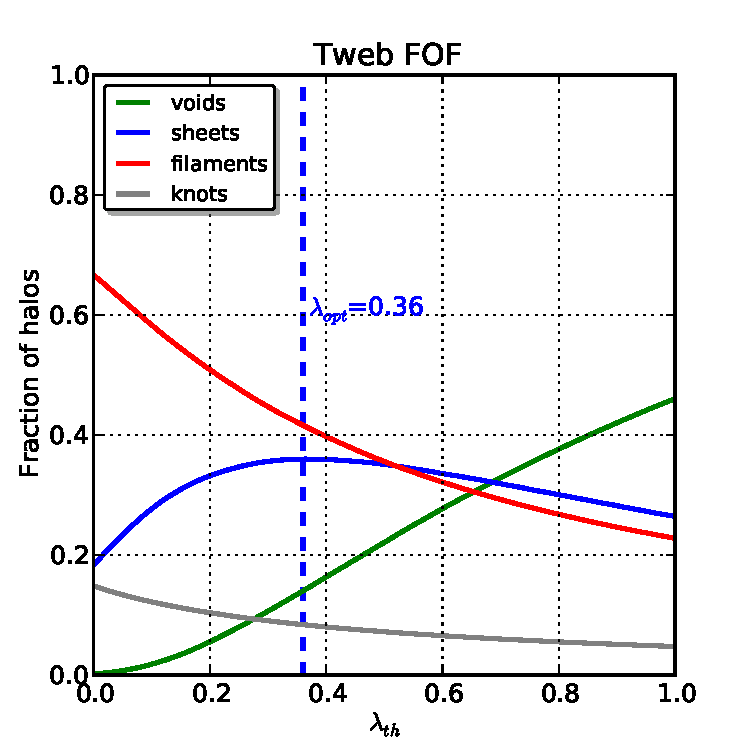
\includegraphics[trim = 0mm 0mm 5mm 5mm, clip, keepaspectratio=true,
  width=0.25\textheight]{./figures/halos_fraction_FOF_Tweb.pdf}  
  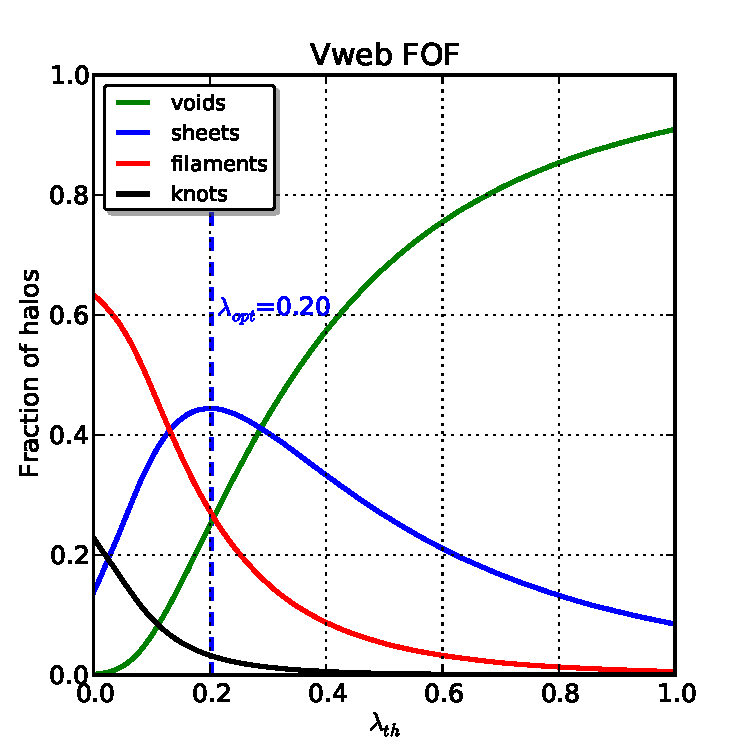
\includegraphics[trim = 0mm 0mm 5mm 5mm, clip, keepaspectratio=true,
  width=0.25\textheight]{./figures/halos_fraction_FOF_Vweb.pdf}

  \captionof{figure}{\small Fractions of halos embedded in each one of 
  the defined environments according to the \lth value. T-web scheme 
  (left panel) and V-web scheme (right panel). The optimal parameters 
  found are $\lambda_{opt}^{T}=0.36$ and $\lambda_{opt}^{V}=0.20$.}

  \label{fig:halos_fractions}
  \vspace{0.1 cm}

\end{figure*}
\end{flushleft}
%.........................................................................


%.........................................................................
%FIGURE 2: Visual impression of the cosmic web
\begin{flushleft}
\begin{figure*}
\centering

  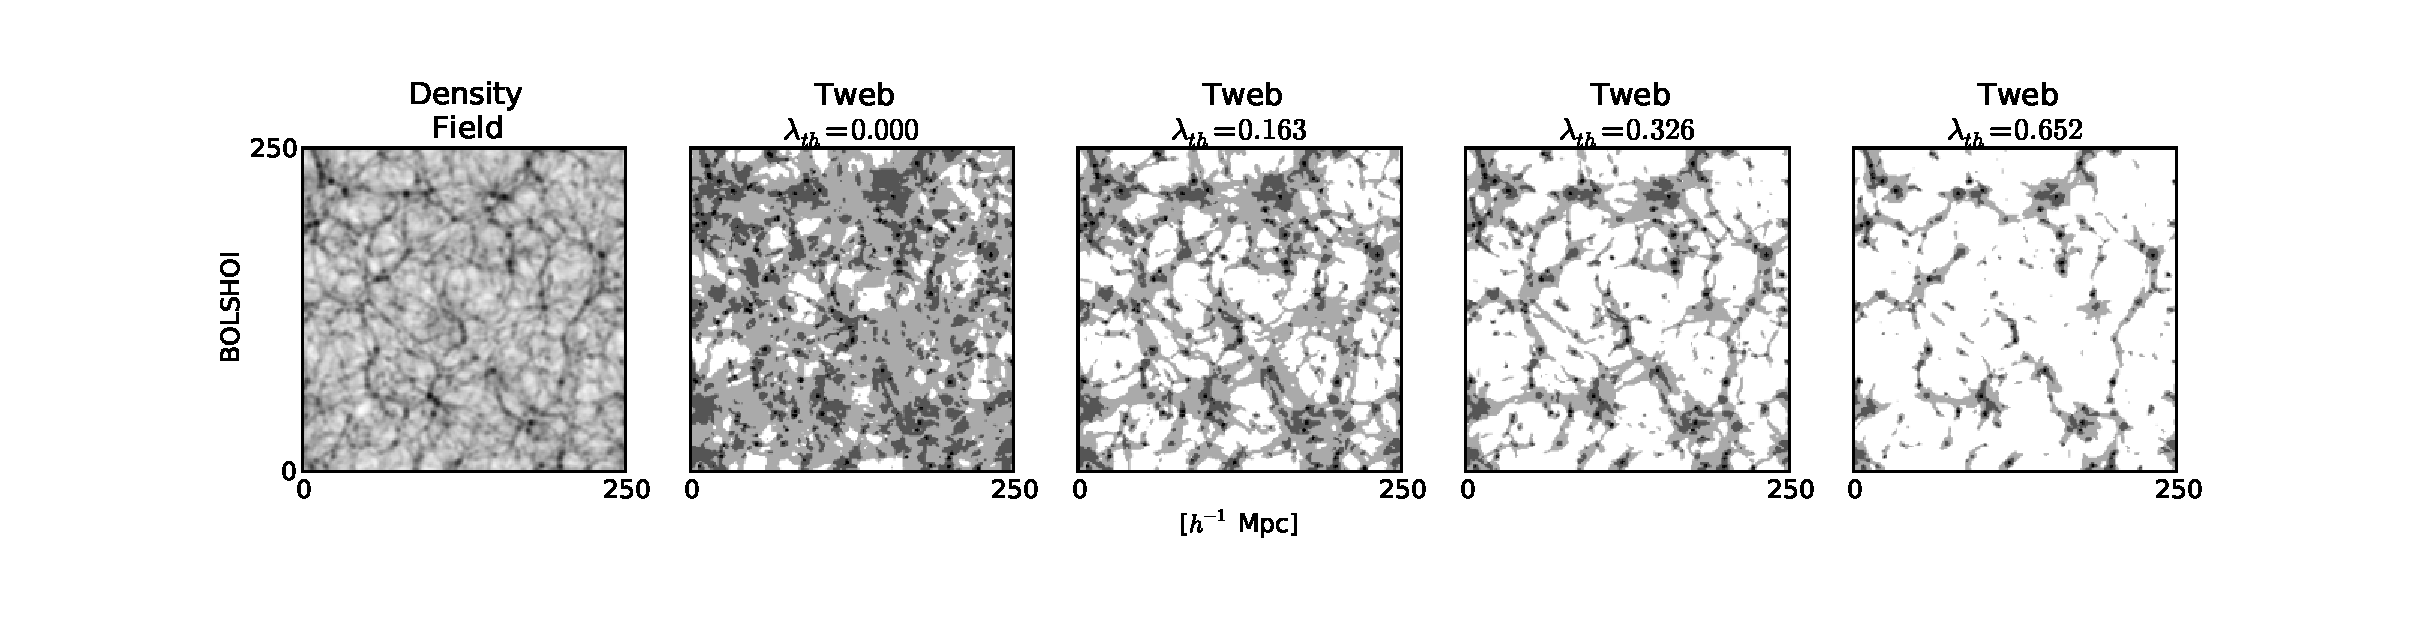
\includegraphics[trim = 42mm 10mm 37mm 10mm, clip, keepaspectratio=true,
  width=0.75\textheight]{./figures/cosmicweb_visual_Tweb.pdf}
  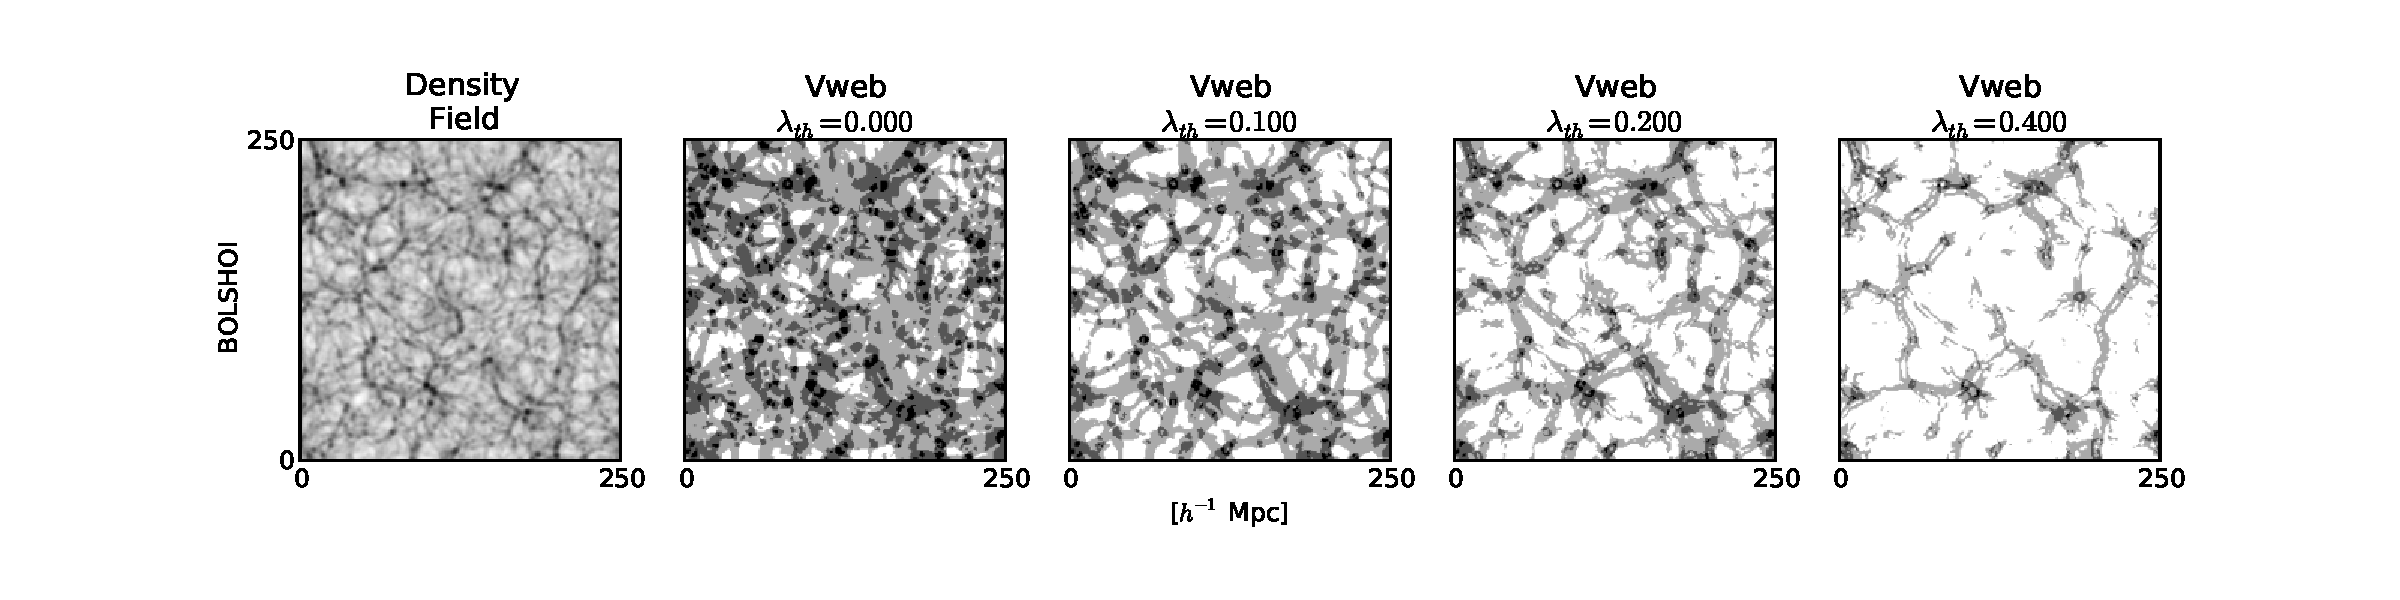
\includegraphics[trim = 42mm 10mm 37mm 10mm, clip, keepaspectratio=true,
  width=0.75\textheight]{./figures/cosmicweb_visual_Vweb.pdf}
  
  \captionof{figure}{\small Visual impression of the density field (left 
  panels), and of each classification scheme with the $\lambda_{th}$ values 
  obtained by our criteria (others panels). The color convention for each 
  environment is (white) - void, (light gray) - sheet, (gray) - filament, 
  (black) - knot. For each web scheme, it has been used the previously 
  established optimal threshold as a reference value, so plots are done 
  with the next values $\lambda_{th} = 0.0$, $\lambda_{th} = 
  \lambda_{opt}/2$, $\lambda_{th} = \lambda_{opt}$ and $\lambda_{th} = 
  2\lambda_{opt}$.}

  \label{fig:visual_impression}
  \vspace{0.1 cm}

\end{figure*}
\end{flushleft}
%.........................................................................


%.........................................................................
%FIGURE 3: Typical mass and pecular velocity
\begin{flushleft}
\begin{figure*}
\centering

  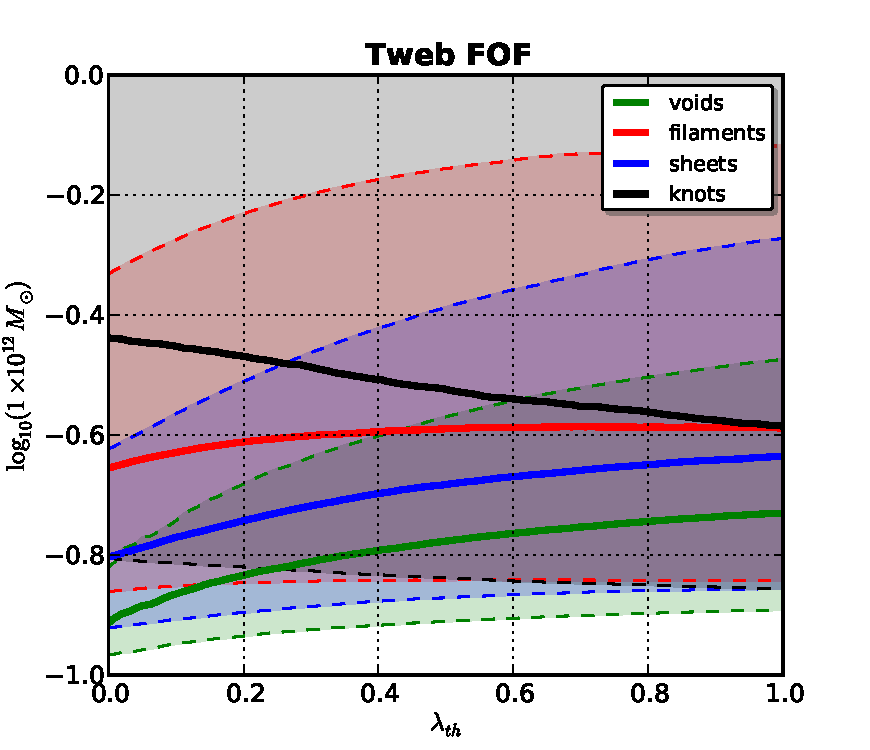
\includegraphics[trim = 0mm 0mm 0mm 0mm, clip, keepaspectratio=true,
  width=0.3\textheight]{./figures/halos_typical_mass_FOF_Tweb.pdf}
  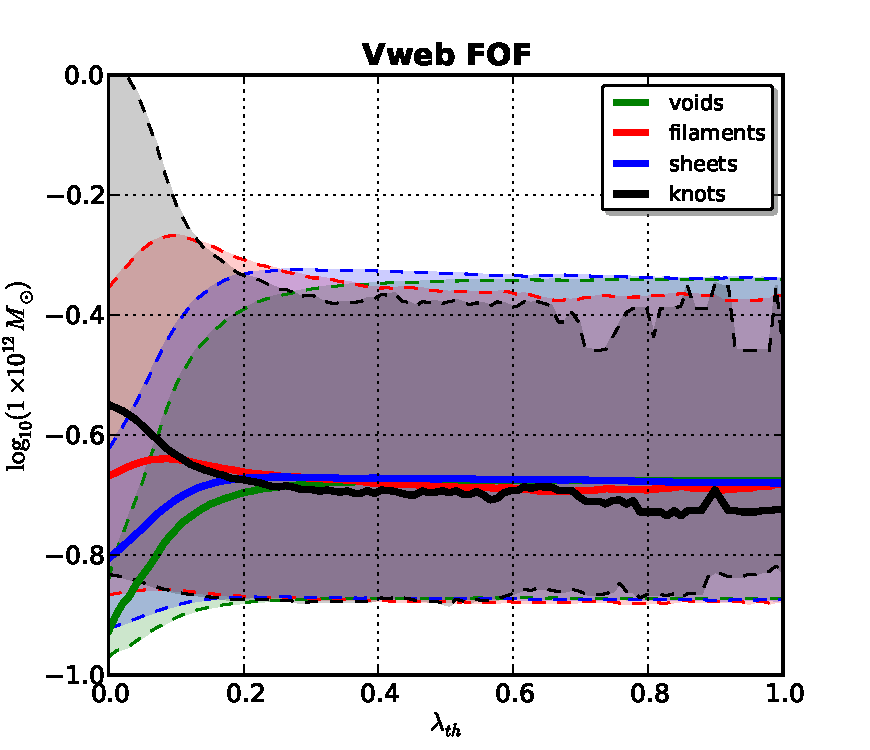
\includegraphics[trim = 0mm 0mm 0mm 0mm, clip, keepaspectratio=true,
  width=0.3\textheight]{./figures/halos_typical_mass_FOF_Vweb.pdf}  
  
  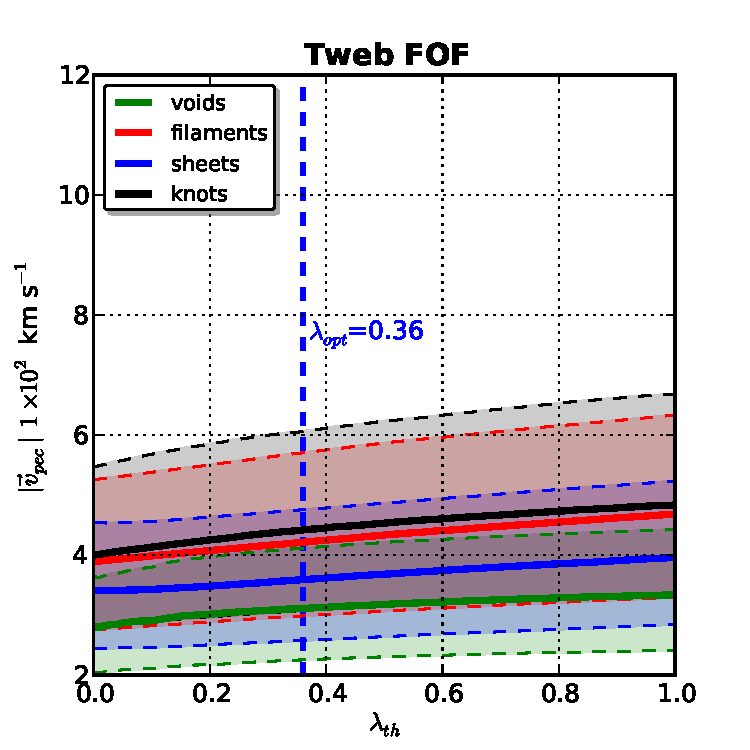
\includegraphics[trim = 0mm 0mm 0mm 0mm, clip, keepaspectratio=true,
  width=0.3\textheight]{./figures/halos_typical_velocity_FOF_Tweb.pdf}
  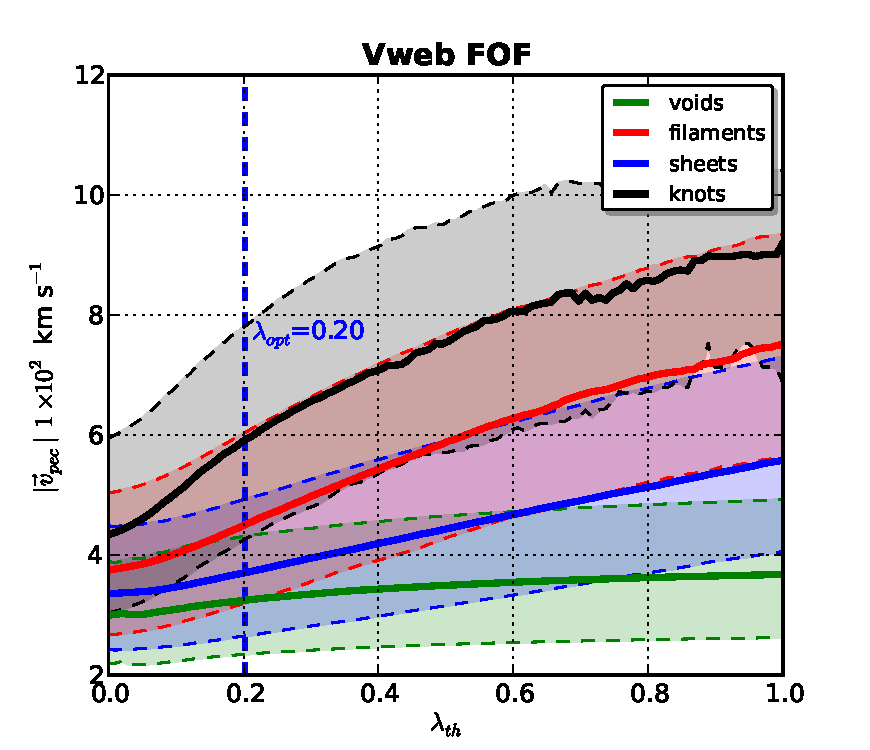
\includegraphics[trim = 0mm 0mm 0mm 0mm, clip, keepaspectratio=true,
  width=0.3\textheight]{./figures/halos_typical_velocity_FOF_Vweb.pdf}  
  
  \captionof{figure}{\small Distribution of masses of dark matter halos
  according the region where they are embedded for both web schemes 
  (upper panels) and of peculiar velocity (lower panels). It can be 
  noticed that the T-web scheme selects different mass ranges according
  to the environment, while the V-web scheme is better selecting ranges
  of peculiar velocity of the dark matter halos. This can be understood
  taking into account the physical origin of each web scheme.}

  \label{fig:typical_mass_velocity}
  \vspace{0.1 cm}

\end{figure*}
\end{flushleft}
%.........................................................................


%.........................................................................
%FIGURE 4: FA and vissual impression
\begin{flushleft}
\begin{figure*}
\centering

  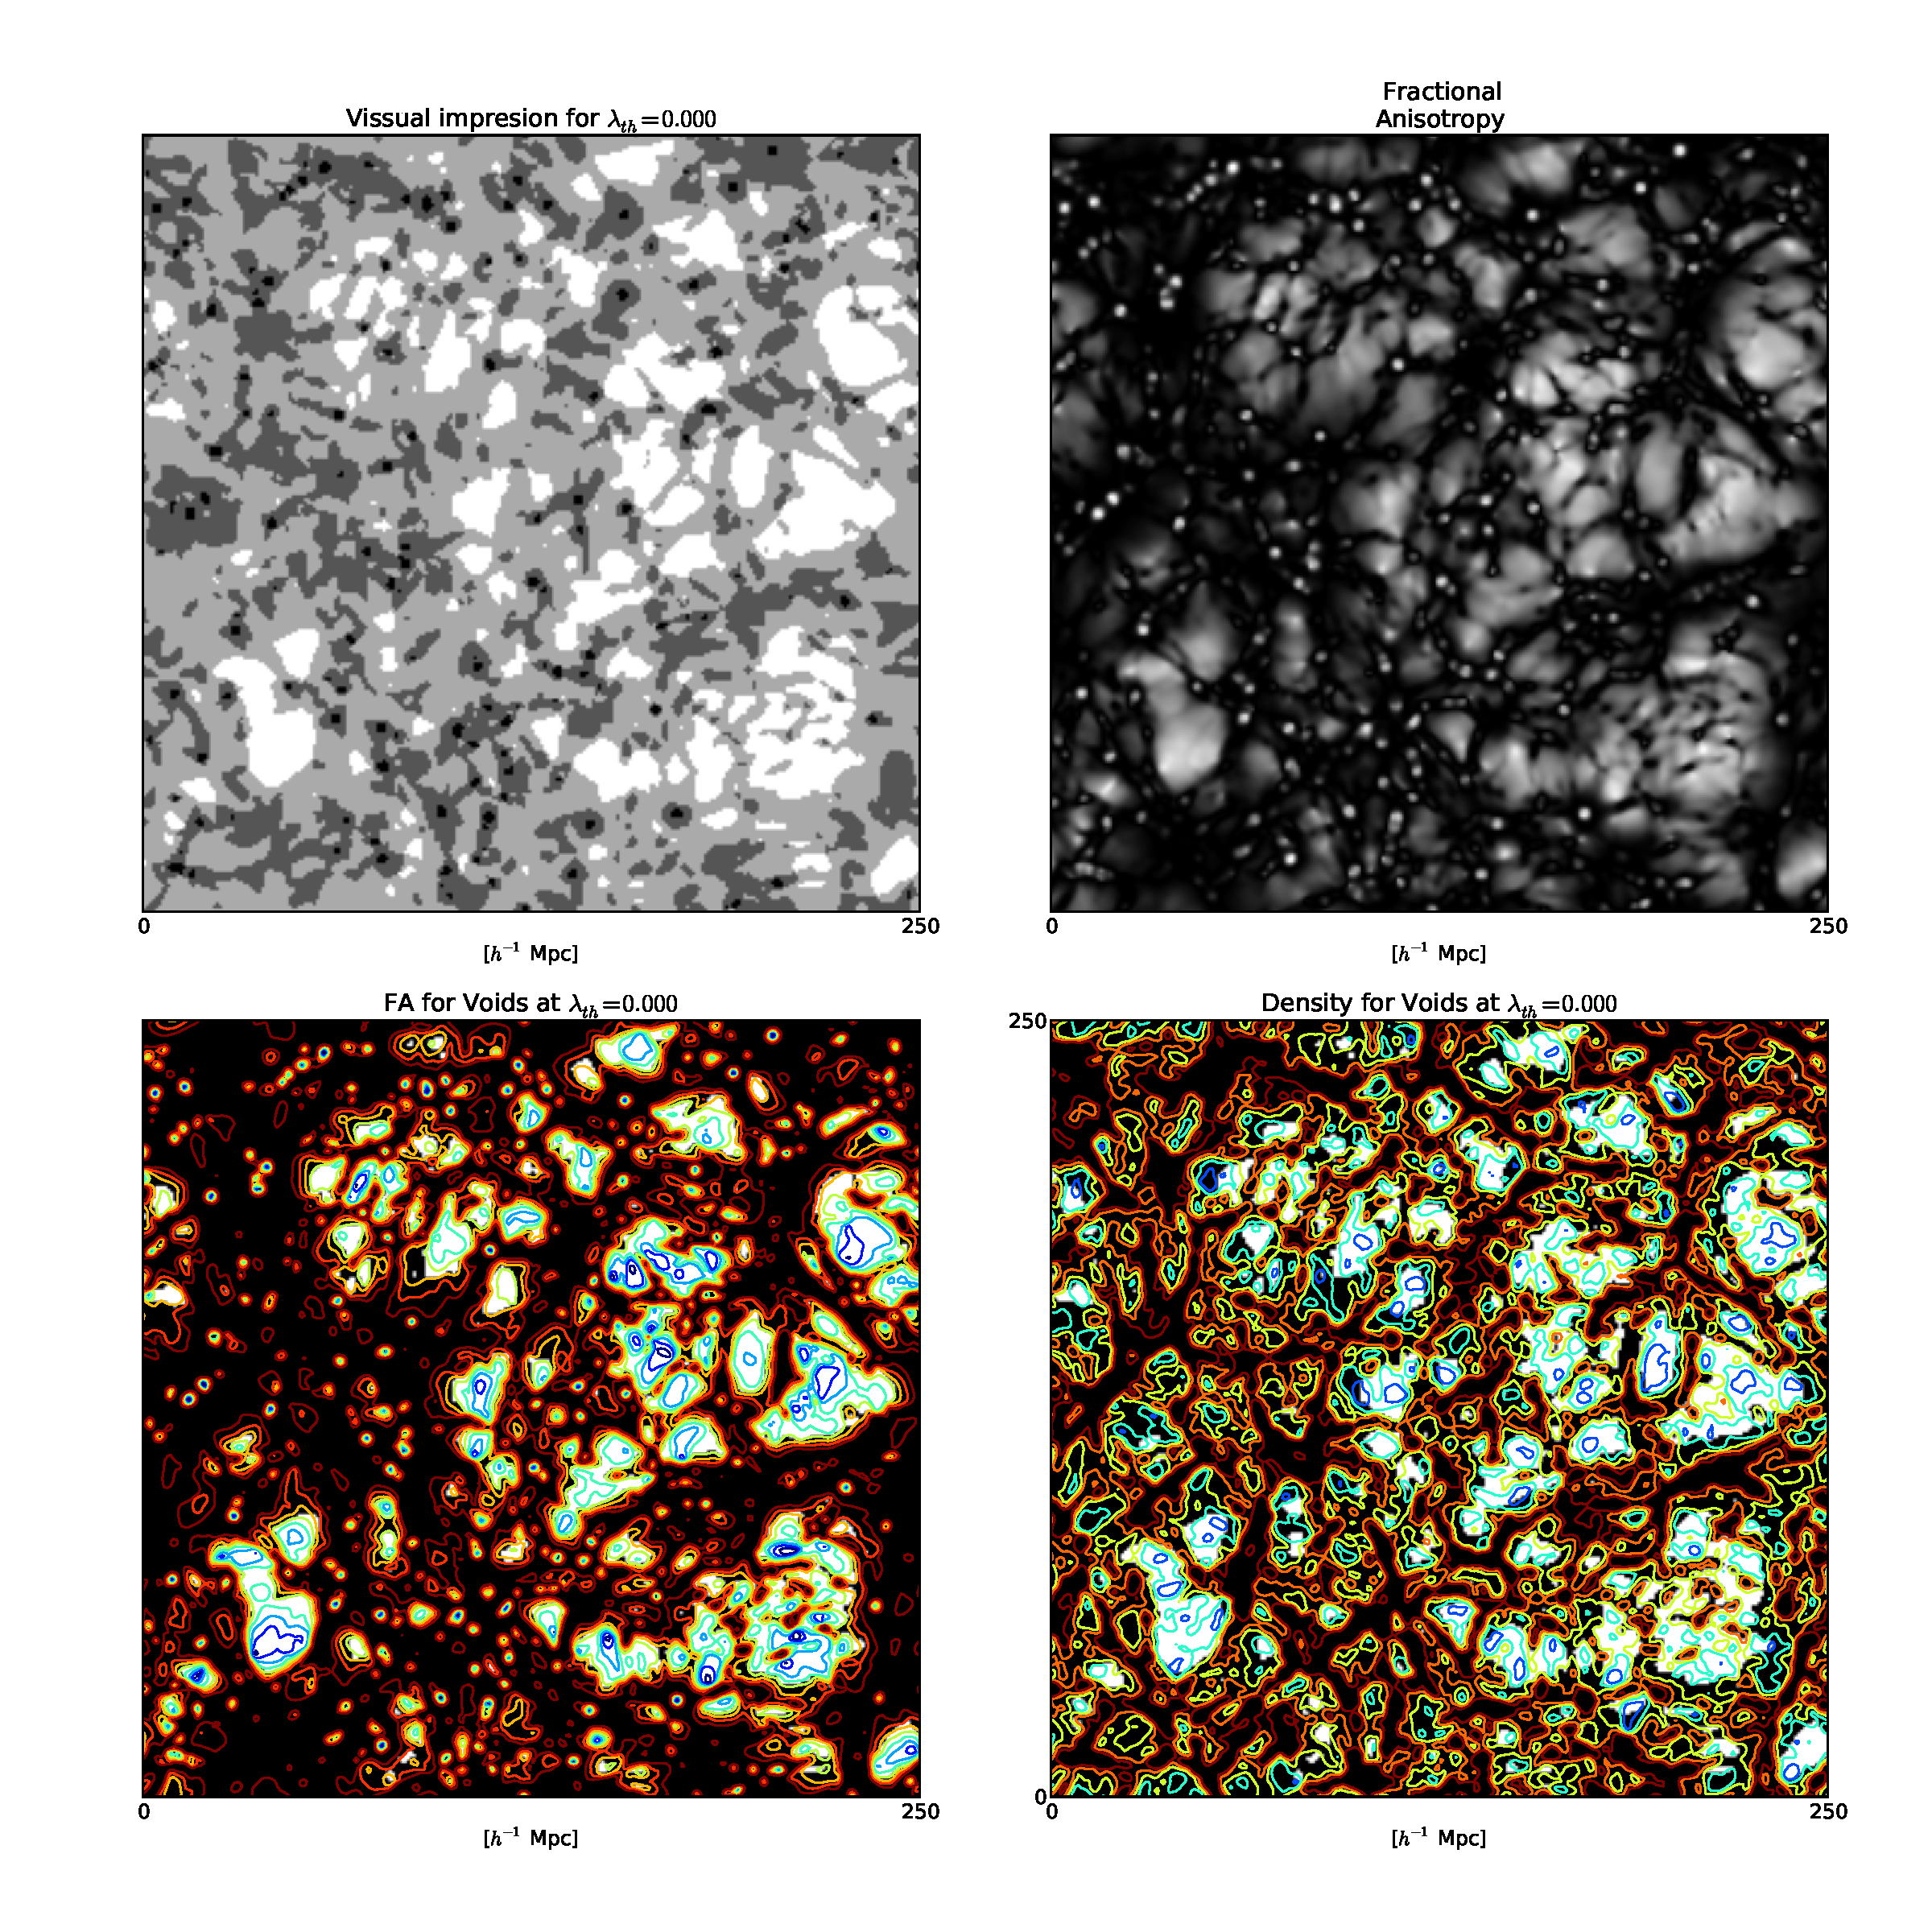
\includegraphics[trim = 25mm 200mm 18mm 15mm, clip, keepaspectratio=true,
  width=0.5\textheight]{./figures/cosmicweb_FA_Tweb(null).pdf}
  
  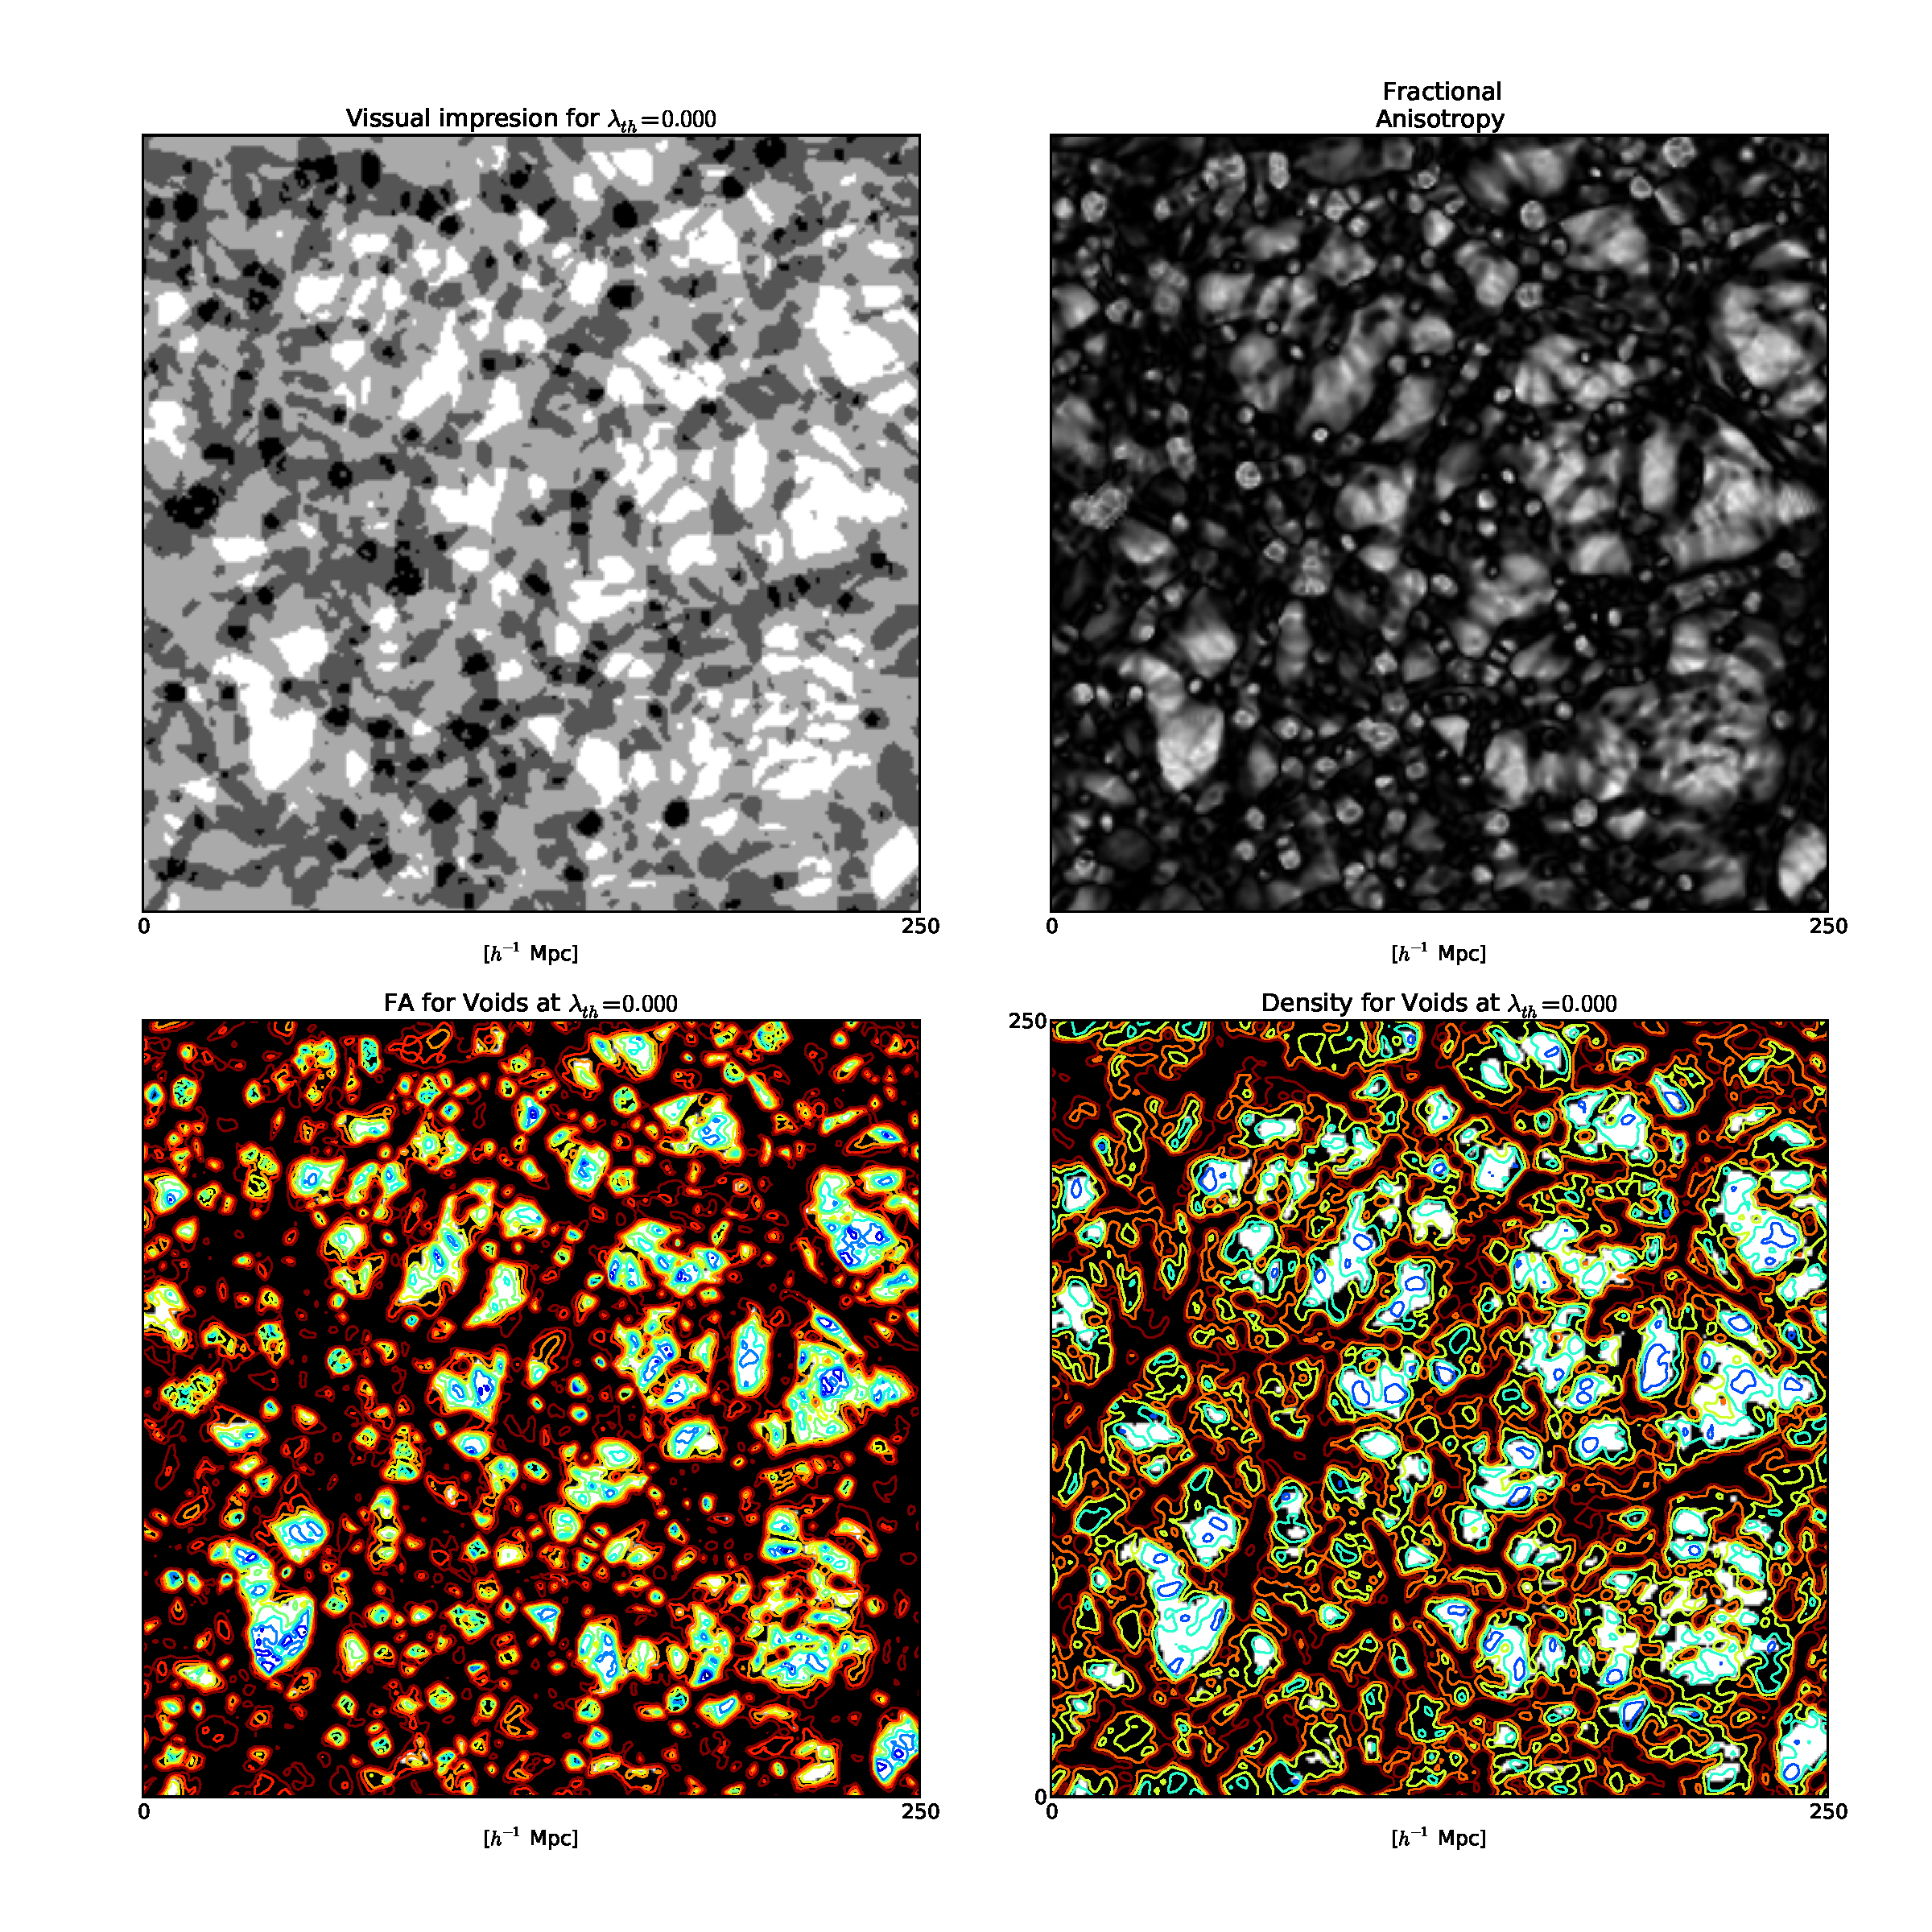
\includegraphics[trim = 25mm 200mm 18mm 15mm, clip, keepaspectratio=true,
  width=0.5\textheight]{./figures/cosmicweb_FA_Vweb(null).pdf}  
  
  \captionof{figure}{\small In left panels is shown the visual impression 
  of the cosmic web for each web scheme (T-web, upper panels. V-web, lower 
  panels) obtained for $\lambda_{th}=0.0$. It can be seen each one of the 
  defined types of environment, where voids corresponds to white zones, 
  sheets to gray, filaments to dark gray and finally knots to black regions. 
  In the right panels is shown the fractional anisotropy field for the same 
  slide of the simulation and for each web schemes, where black regions 
  correspond to FA$=1$ and white regions to FA$=0$. It can be noticed the 
  degeneration of low values of FA for knots and central regions of voids, 
  while high values of FA (FA $\lesssim 1$) are consistent with filaments 
  and highly planar sheets.}

  \label{fig:FA_field}
  \vspace{0.1 cm}

\end{figure*}
\end{flushleft}
%.........................................................................


%.........................................................................
%FIGURE 5: Distributions of FA and density regarding the Lambda_1 eigenvalue
\begin{flushleft}
\begin{figure*}
\centering

  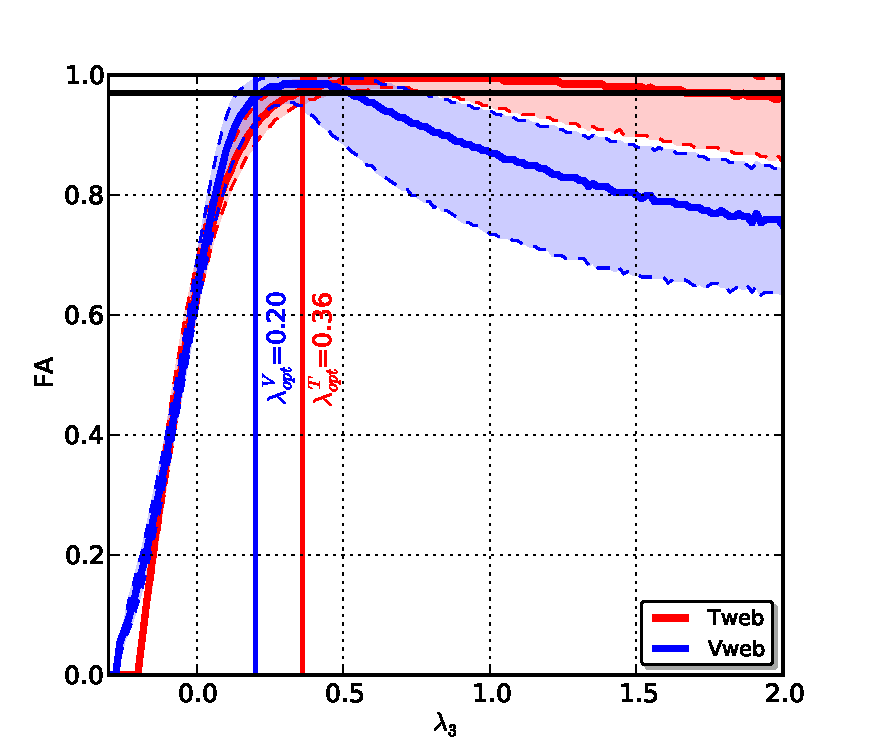
\includegraphics[trim = 2mm 2mm 5mm 10mm, clip, keepaspectratio=true,
  width=0.3\textheight]{./figures/FA_L1.pdf}
  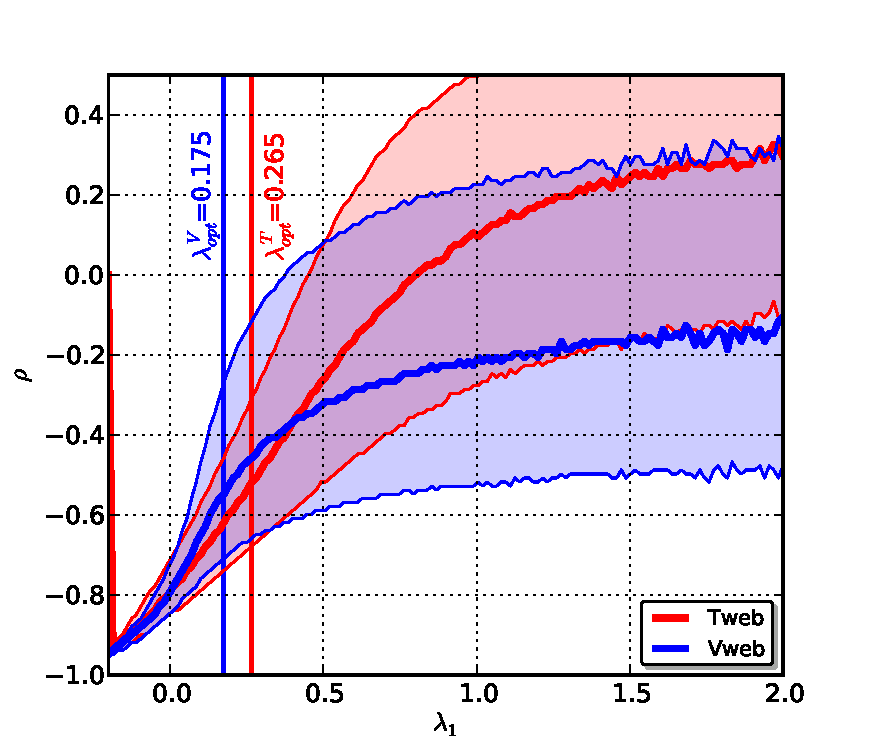
\includegraphics[trim = 2mm 2mm 5mm 10mm, clip, keepaspectratio=true,
  width=0.3\textheight]{./figures/delta_L1.pdf}  
  
  \captionof{figure}{\small In this figure is shown the distribution of the
  fractional anisotropy (left panel) and density field (right panel) with 
  respect to the eigenvalue $\lambda_1$ for each web scheme (T-web, red 
  lines. V-web, blue lines) as calculated over all the cells of the grid.
  Thick central lines correspond to the median of the distribution and 
  coloured regions to the $50\%$ of the cells, delimited by quartiles 
  $Q_1$ and $Q_3$.}

  \label{fig:L1_correlations}
  \vspace{0.1 cm}

\end{figure*}
\end{flushleft}
%.........................................................................


%.........................................................................
%FIGURE 6: Distributions of local mimima
\begin{flushleft}
\begin{figure*}
\centering

  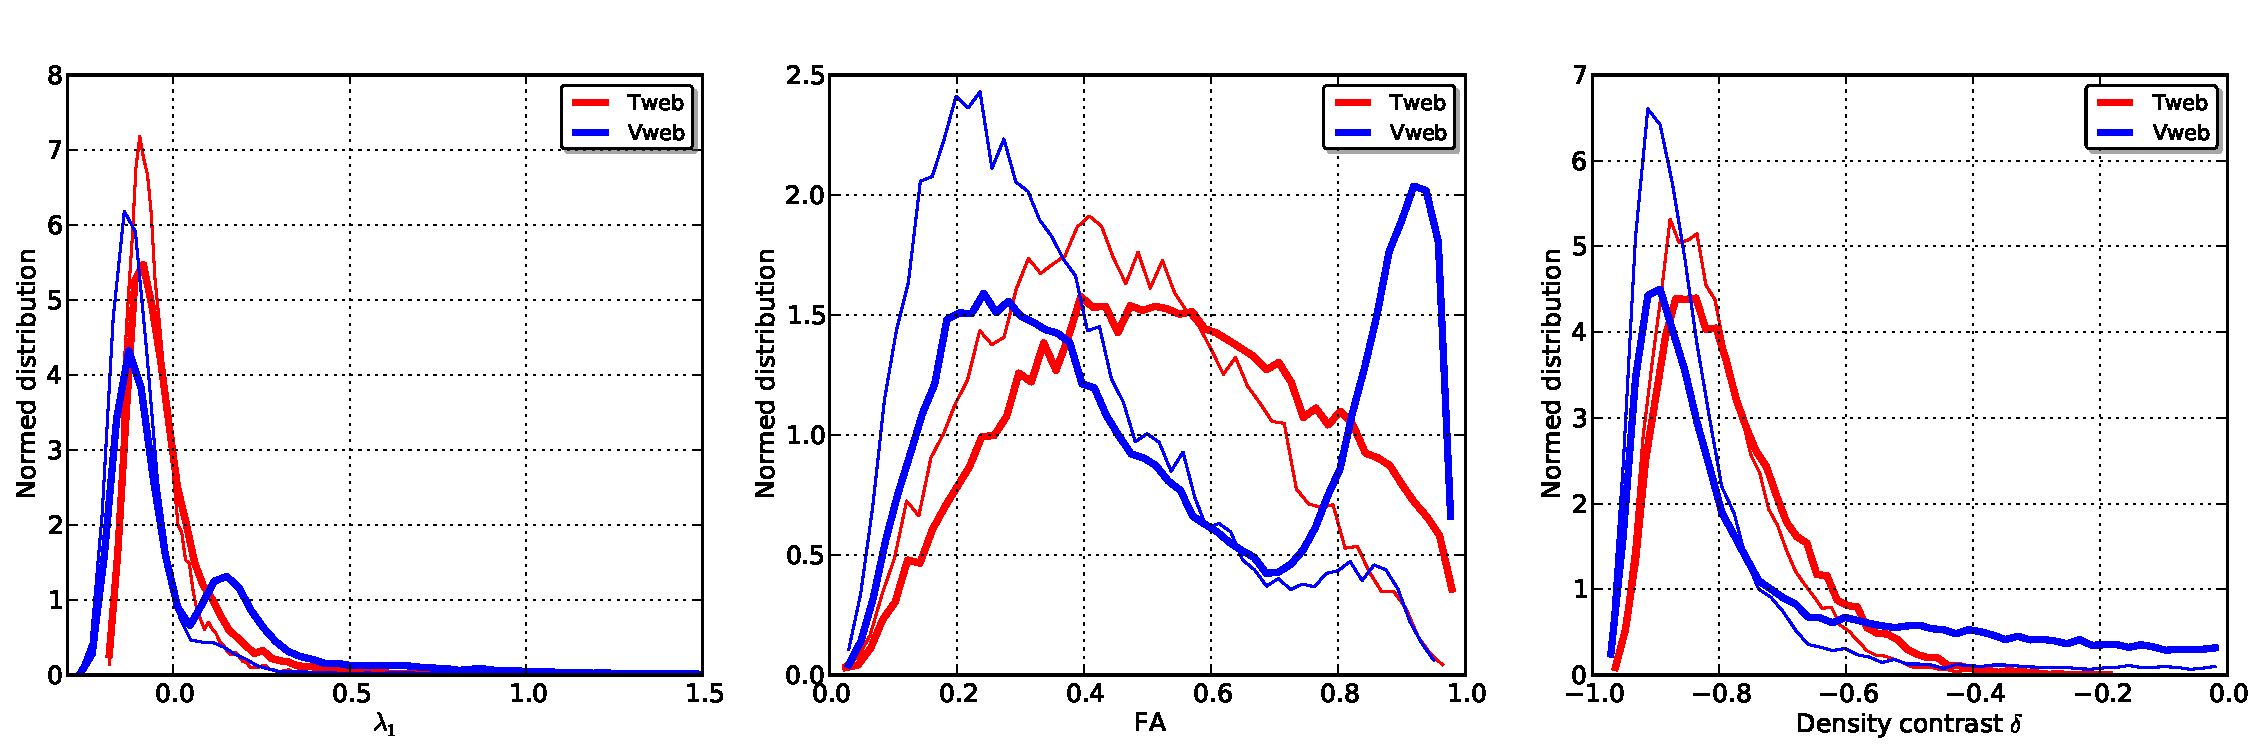
\includegraphics[trim = 0mm 2mm 0mm 2mm, clip, keepaspectratio=true,
  width=0.7\textheight]{./figures/central_voids.pdf}
  
  \captionof{figure}{\small In this figure is shown the distribution of the
  fractional anisotropy (left panel) and density field (right panel) with 
  respect to the eigenvalue $\lambda_1$ for each web scheme (T-web, red 
  lines. V-web, blue lines) as calculated over all the cells of the grid.
  Thick central lines correspond to the median of the distribution and 
  coloured regions to the $50\%$ of the cells, delimited by quartiles 
  $Q_1$ and $Q_3$.}

  \label{fig:L1_correlations}
  \vspace{0.1 cm}

\end{figure*}
\end{flushleft}
%.........................................................................


\end{document}
